\documentclass{article}
\usepackage{amsmath}
\usepackage{graphicx}
\usepackage{fancyhdr}
\usepackage{array}
\usepackage{booktabs}
\usepackage[sorting=none]{biblatex}
\usepackage[margin=1in]{geometry}
\usepackage{listings}

\lstset{
    language=Python,                    % تنظیم زبان پایتون
    backgroundcolor=\color{white},      % رنگ پس‌زمینه سفید
    basicstyle=\ttfamily\footnotesize,  % استفاده از فونت monospaced
    keywordstyle=\color{blue},           % رنگ کلمات کلیدی
    commentstyle=\color{green},         % رنگ کامنت‌ها
    stringstyle=\color{red},            % رنگ رشته‌ها
    numbers=left,                       % شماره‌گذاری خطوط
    numberstyle=\tiny\color{gray},      % استایل شماره‌های خطوط
    stepnumber=1,                       % شماره‌گذاری هر خط
    numbersep=5pt,                      % فاصله شماره‌گذاری از کد
    showspaces=false,                   % نمایش فضاها
    showstringspaces=false,             % نمایش فضاها در رشته‌ها
    showtabs=false,                     % نمایش تب‌ها
    frame=single,                       % نمایش قاب دور کد
    rulecolor=\color{black},            % رنگ قاب دور کد
    tabsize=2,                          % اندازه تب‌ها
    captionpos=b,                       % عنوان در پایین قرار می‌گیرد
    breaklines=true,                    % تقسیم خط‌های طولانی
    breakatwhitespace=true              % تقسیم در فضای خالی
}
\usepackage[hidelinks]{hyperref}
\usepackage{subfigure}
\hypersetup{
    colorlinks=true,
    linkcolor=teal,
    filecolor=magenta,      
    urlcolor=teal,
    citecolor = teal
    }
\usepackage{xcolor}
\usepackage{xepersian}
\usepackage{fontspec}
\setlength\headheight{28pt} 
\addbibresource{bibliography.bib}
\settextfont[Scale=1.2]{IRLotus.TTF}
\setlatintextfont[Scale=1]{Times New Roman}
\renewcommand{\baselinestretch}{1.5}
\pagestyle{fancy}
\fancyhf{}
\rhead{
\includegraphics[width=1cm]{FaultD.png}امتحان میانترم درس یادگیری ماشین}
\lhead{\thepage}
\lfoot{علیرضا امیری}
\renewcommand{\headrulewidth}{1pt}
\renewcommand{\footrulewidth}{1pt}
\AtBeginDocument{
	\def\chapterautorefname{فصل}%
	\def\sectionautorefname{پاسخ سوال}%
	\def\subsectionautorefname{بخش}%
	\def\subsubsectionautorefname{بخش}%
	\def\equationautorefname{رابطهٔ}%
    \def\lstlistingautorefname{برنامۀ}%
}
\renewcommand{\lstlistingname}{Code}
\begin{document}

\begin{titlepage}
\begin{center}

  \begin{figure}[h!]
 	\centering
 	\subfigure{
 		
\includegraphics[width=0.43\columnwidth]{KNTULogo.pdf}
 		\label{fig:FD3M4sav43i22ngCdW2}
 	}
 	\subfigure
 	{
 		
\includegraphics[width=0.33\columnwidth, height=0.45\columnwidth]{Fault}
 		\label{fig:FD3Msav43i22ngCdW2}
 	}
 \end{figure}
 
 % 
\includegraphics[width=0.5\textwidth]{KNTULogo.pdf}\\
 
\vfill
        
\Huge
\textbf{یادگیری ماشین}\\
\textbf{آزمون میان ترم}\\
        
\vfill
        
\begin{table}[ht]
    \centering
    \huge
    \begin{tabular}{|c|c|}
    \hline
    نام و نام خانوادگی & علیرضا امیری\\
    \hline
    شمارۀ دانشجویی &  40202414\\
    \hline
    تاریخ & خرداد ماه 1404\\
    \hline
    \end{tabular}
\end{table}
\end{center}
\end{titlepage}



\tableofcontents

\section{پاسخ سوال هماهنگ شده اول}
برای کلاس بندی دو دسته داده که هر یک دارای توزیع نرمال گوسی با میانگین $\mu$، کوواریانس $\sigma$ و ویژگی های $x$ هستند، از روابط احتمالی این توزیع ها و تعریف توزیع نرمال به شرح زیر استفاده می کنیم.
\begin{equation}
	p(\mathbf{x}\mid C_i)
	= \mathcal{N}\bigl(\mathbf{x};\boldsymbol\mu_i,\Sigma_i\bigr)
	= \frac{1}{(2\pi)^{d/2}\,\lvert\Sigma_i\rvert^{1/2}}
	\exp\!\Bigl(-\tfrac12(\mathbf{x}-\boldsymbol\mu_i)^\top\Sigma_i^{-1}(\mathbf{x}-\boldsymbol\mu_i)\Bigr),
	\quad i=1,2.
\end{equation}

حال، برای دسته بندی این دو کلاس، طبق رابطه ی زیر با استفاده از لگاریتم likelihood،و با فرض $P(C_1)=P(C_2)$ خواهیم داشت:
\begin{equation}
	  \delta(\mathbf{x})
	=\ln p(\mathbf{x}\mid C_1)\;-\;\ln p(\mathbf{x}\mid C_2)
	\;<>_{C_2}^{C_1}0.
\end{equation} 

با جایگذاری فرم گوسی داده ها در این رابطه، رابطه ی تصمیم گیری به فرم کوادراتیک به صورت زیر به دست می آید:
\begin{equation}
	\begin{aligned}
		\delta(\mathbf{x})
		&=\Bigl[-\tfrac12(\mathbf{x}-\boldsymbol\mu_1)^\top\Sigma_1^{-1}(\mathbf{x}-\boldsymbol\mu_1)
		-\tfrac12\ln|\Sigma_1|\Bigr]\\
		&\quad -\Bigl[-\tfrac12(\mathbf{x}-\boldsymbol\mu_2)^\top\Sigma_2^{-1}(\mathbf{x}-\boldsymbol\mu_2)
		-\tfrac12\ln|\Sigma_2|\Bigr]\\
		&=-\tfrac12(\mathbf{x}-\boldsymbol\mu_1)^\top\Sigma_1^{-1}(\mathbf{x}-\boldsymbol\mu_1)
		+\tfrac12(\mathbf{x}-\boldsymbol\mu_2)^\top\Sigma_2^{-1}(\mathbf{x}-\boldsymbol\mu_2)
		-\tfrac12\ln\frac{|\Sigma_1|}{|\Sigma_2|}.
	\end{aligned}
\end{equation}
\begin{equation}
	\mathbf{x}^\top\bigl(\Sigma_2^{-1}-\Sigma_1^{-1}\bigr)\mathbf{x}
	+2\bigl(\boldsymbol\mu_1^\top\Sigma_1^{-1}-\boldsymbol\mu_2^\top\Sigma_2^{-1}\bigr)\mathbf{x}
	+c
	, 
	c=\boldsymbol\mu_2^\top\Sigma_2^{-1}\boldsymbol\mu_2
	-\boldsymbol\mu_1^\top\Sigma_1^{-1}\boldsymbol\mu_1
	-\ln\frac{|\Sigma_2|}{|\Sigma_1|}.
\end{equation}
که با در نظر داشتن متغیر ویژگی های $x$ و عبارت $\mathbf{x} \mathbf{x}^\top = \mathbf{x}^2
$ فرمت کوادراتیک این معادله مشخص میشود. حال، با تغییر مقادیر میانگین و کوواریانس، می توانیم سطوح مختلفی را به دست بیاوریم. به عنوان مثال، در صورتی که مقادیر کوواریانس دو کلاس با یکدیگر برابر باشد، آنگاه $\Sigma_1=\Sigma_2=\Sigma$ و در نتیجه $\Sigma_2^{-1}-\Sigma_1^{-1}=0$ و در نهایت با حذف ضریب بخش درجه 2 این معادله، صفحه ی تصمیم به فرمت خطی به صورت زیر به دست می آید:
\begin{equation}
	(\boldsymbol\mu_1-\boldsymbol\mu_2)^\top\Sigma^{-1}\,\mathbf{x}
	\;-\;\tfrac12\bigl(\boldsymbol\mu_1^\top\Sigma^{-1}\boldsymbol\mu_1
	-\boldsymbol\mu_2^\top\Sigma^{-1}\boldsymbol\mu_2\bigr)
	=0,
\end{equation}

به عنوان مثال، حالت های مختلف برای تغییرات میانگین و کوواریانس داده های کلاس ها در 
\autoref{fig:1}
رسم شده است.
\begin{figure}[h!]
	\centering
	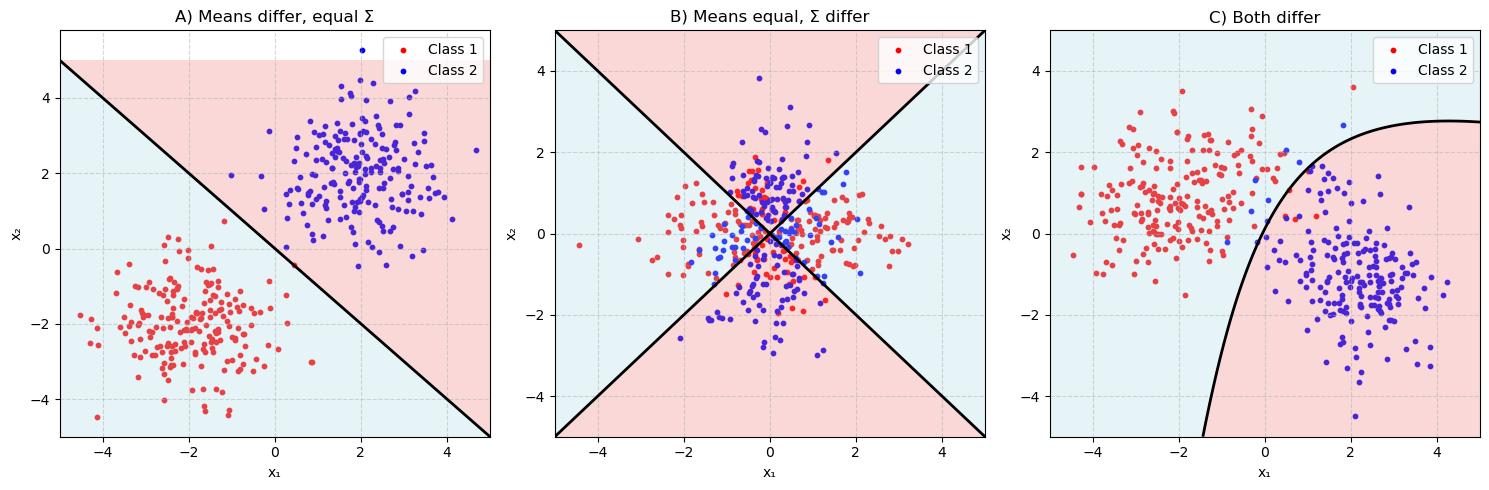
\includegraphics[width=1\linewidth]{1}
	\caption{وضعیت های مختلف صفحه تصمیم با تغییر میانگین و کوواریانس}
	\label{fig:1}
\end{figure}

\section{پاسخ سوال هماهنگ شده دوم}
در صورتی که تابع توزیع احتمال را در اختیار داشته باشیم، اولین گام برای تولید نمونه هایی که دارای توزیعی مطابق با این تابع باشند، محاسبه ی تابع توزیع احتمال تجمعی یا به اختصار CDF است. بنابراین، ابتدا با محاسبه ی انتگرال، این تابع را محاسبه می کنیم:
\begin{equation}
	F(x) = \int_{-\infty}^{x} f(t) dt
\end{equation}
آنگاه با استفاده از وارون تابع CDF و وارد کردن داده های تصادفی به آن، داده هایی با توزیع مورد نظر بسازیم. این فرایند به طریق زیر انجام خواهد شد:
\begin{equation}
	x = F^{-1}(u) \Rightarrow x \sim f(x)
\end{equation}
برای راحتی در این بخش، می توان داده های تصادفی را با استفاده از دستور $Uniform(0,1)$ ایجاد کرد. در این حالت، با جایگذاری این داده ها به عنوان ورودی $ F^{-1}(u)$، می توانیم داده های مورد نظر را به دست بیاوریم. با این حال، این روش تنها در حالتی برقرار است که بتوانیم از CDF به دست آمده وارون بگیریم که این در همه ی شرایط برقرار نیست. علاوه بر این، فرایند تولید اعداد با توزیع یکنواخت نیز در اینجا توضیح داده نشده است که در ادامه به آن خواهیم پرداخت.
برای ساخت اعداد تصادفی، الگوریتم های مختلفی مانند $Linear Congruential Generator (LCG)$ و $Mersenne Twister$ تولید می شوند. در این الگوریتم ها، اعداد رندوم در بازه ی 0 تا 1 از تقسیم عددی بزرگ بر $ F^{32}$ یا $ F^{64}$ به دست می آیند. در اینجا، عددی که بر این مقدار تقسیم می شود با استفاده از پارامترهای تصادفی در سخت افزار کامپیوتر ایجاد می شود.

\section{پاسخ سوال 1}

\section{پاسخ سوال 2}

\section{پاسخ سوال 3}

\section{پاسخ سوال 4}





\end{document}

